%!TEX root = ../main.tex
\section{Homework \thesection}

\subsection{Color Histogram Features}
Implement the missing body of code in \href{./hw5/histvec.m}{\texttt{histvec.m}}, which creates a color histogram feature vector.
Follow the comments in the code for the details.
We call this with \texttt{C = reduce(im,C,S);}.
Run \href{./hw5/q1.m}{\texttt{q1.m}}, which will generate an output image \href{./hw5/q1_result.png}{q1\_result.png}.
Include this output in the writeup.
Also include the code as plain text.
Also, inspect the code in \href{./hw5/q1.m}{\texttt{q1.m}} and answer the following question in one sentence: Describe the object in the image that is covered by the superpixel used to compute the histograms in \href{./hw5/q1.m}{\texttt{q1.m}}.
\lstinputlisting[style=Matlab-editor]{./hw5/histvec.m}
The object with index 88 is a yellow (orange) pepper.
\begin{figure}[htbp]
	\centering
	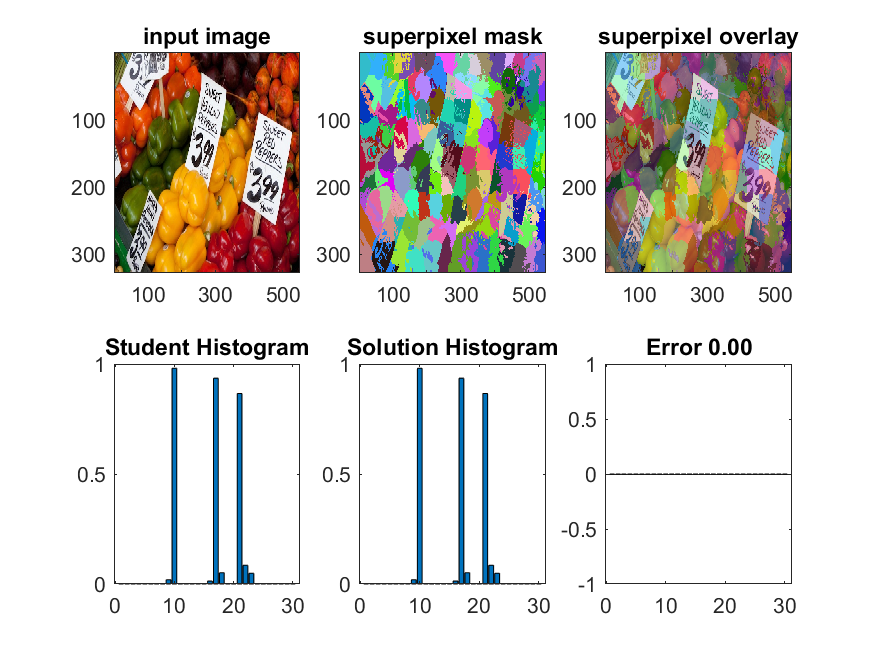
\includegraphics[width=\textwidth]{hw5/q1_result.png}
    \caption{Color histogram features \href{./hw5/q1_result.png}{q1\_result.png}}
    \label{fig:17}
\end{figure}

\subsection{Superpixel Adjacency}
\begin{enumerate}
    \item Implement the missing body of code in \href{./hw5/segNeighbors.m}{\texttt{segNeighbors.m}}, which computes the adjacency matrix for the superpixel     graph.
    Follow the comments in the code for the details.
    We call this in the graph cuts code.
    Run \href{./hw5/q2.m}{\texttt{q2.m}}, which will generate an output image \href{./hw5/q2_result.png}{q2\_result.png}.
    Include this output in the writeup.
    Also include the code as plain text.
    \item Implement a small function to compute the average node degree.
    Include the code as plain text in the writeup.
    \item Why is the adjacency graph not a perfect banded diagonal matrix?
\end{enumerate}
\subsubsection{Adjacency Matrix}
\lstinputlisting[style=Matlab-editor]{./hw5/segNeighbors.m}
\begin{figure}[htbp]
	\centering
	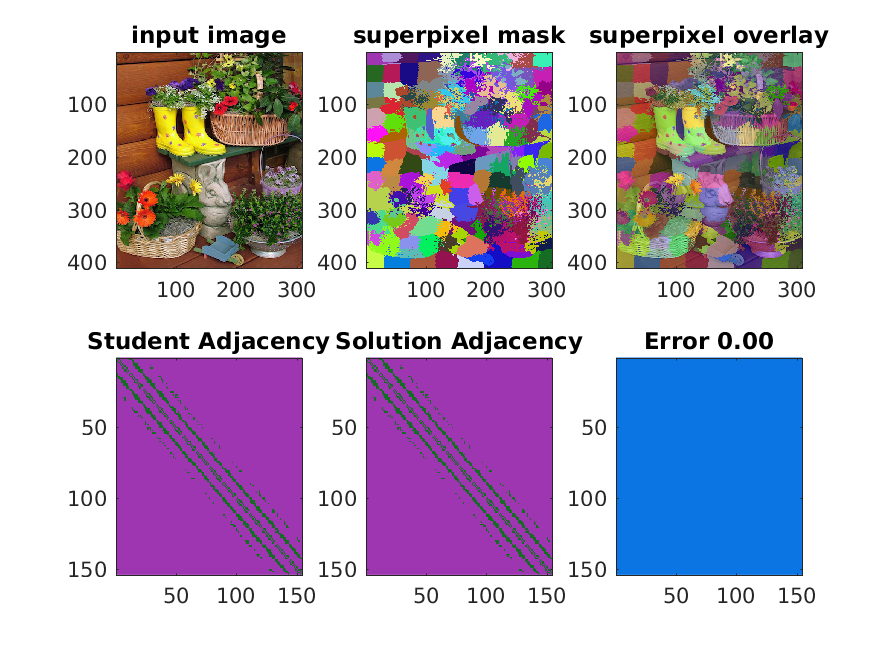
\includegraphics[width=\textwidth]{hw5/q2_result.png}
    \caption{Superpixel adjacency \href{./hw5/q2_result.png}{q2\_result.png}}
    \label{fig:18}
\end{figure}
\subsubsection{Average Node Degree}
% Average node degree is the sum of the adjacency matrix divided by its size.
\lstinputlisting[style=Matlab-editor]{./hw5/avgnodegree.m}
\subsubsection{Adjacency Graph}
The adjacency graph almost never banded, and if there is at least an edge in the graph, the adjacency matrix is never banded.
This is because the diagonal entries are zeros by definition, and if there is an edge, there is a non-zero element off the main diagonal.
Furthermore, whether the graph has nonzero entries close to the diagonal depends on the permutation of the index.
If we rename the index, the nonzero elements can be closer to the diagonal.


\subsection{Graph-Cuts}
\begin{enumerate}
    \item Implement the missing two bodies of code in \href{./hw5/graphcut.m}{\texttt{graphcut.m}}, which
    \begin{itemize}
    \item creates the graph by defining the capacity matrix and 
    \item extract the results after running the max-flow/min-cut method.
    \end{itemize}
    See the comments and refer to class notes for details.
    Run \href{./hw5/q3.m}{\texttt{q3.m}}, which will generate an output image \href{./hw5/q3_result.png}{q3\_result.png}.
    Include this output and the full implementation as plain
    text in your writeup.
    \item Using the debugger, save an image of your capacity matrix before running graph cuts in \href{./hw5/q3.m}{\texttt{q3.m}} and submit it.
    In a few sentences, relate the adjacency matrix to the capacity image.
    Be sure to cover all nodes of the graph in your description.
    \item Please explain why the capacity between adjacent nodes in the graph that have resulted from superpixels is downweighted with respect to the capacity between nodes in the graph and the special source and sink nodes.
\end{enumerate}
\subsubsection{Filling Capacity Matrix}
\lstinputlisting[style=Matlab-editor]{./hw5/graphcut.m}
\begin{figure}[htbp]
	\centering
	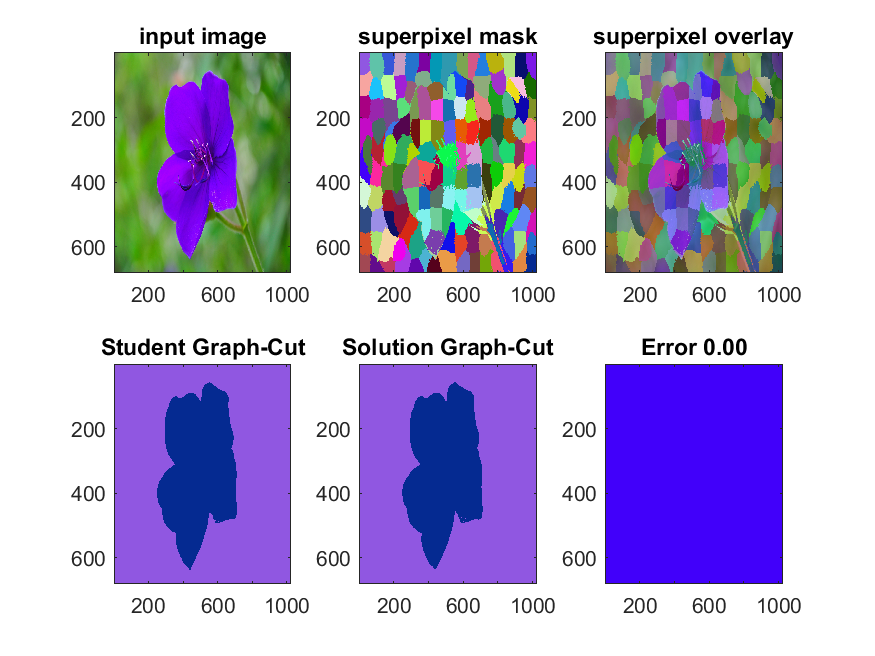
\includegraphics[width=\textwidth]{hw5/q3_result.png}
    \caption{Graph cut \href{./hw5/q3_result.png}{q3\_result.png}}
    \label{fig:19}
\end{figure}
\subsubsection{Capacity Matrix Graph}
The capacity matrix has some non-zero values where the adjacency matrix is 1.
The extra row which represents the source have more non-zero values, and the extra column which represents the sink also have more non-zero values.
The capacity matrix graph is plotted in Figure \ref{fig:20}.
\begin{figure}[htbp]
	\centering
	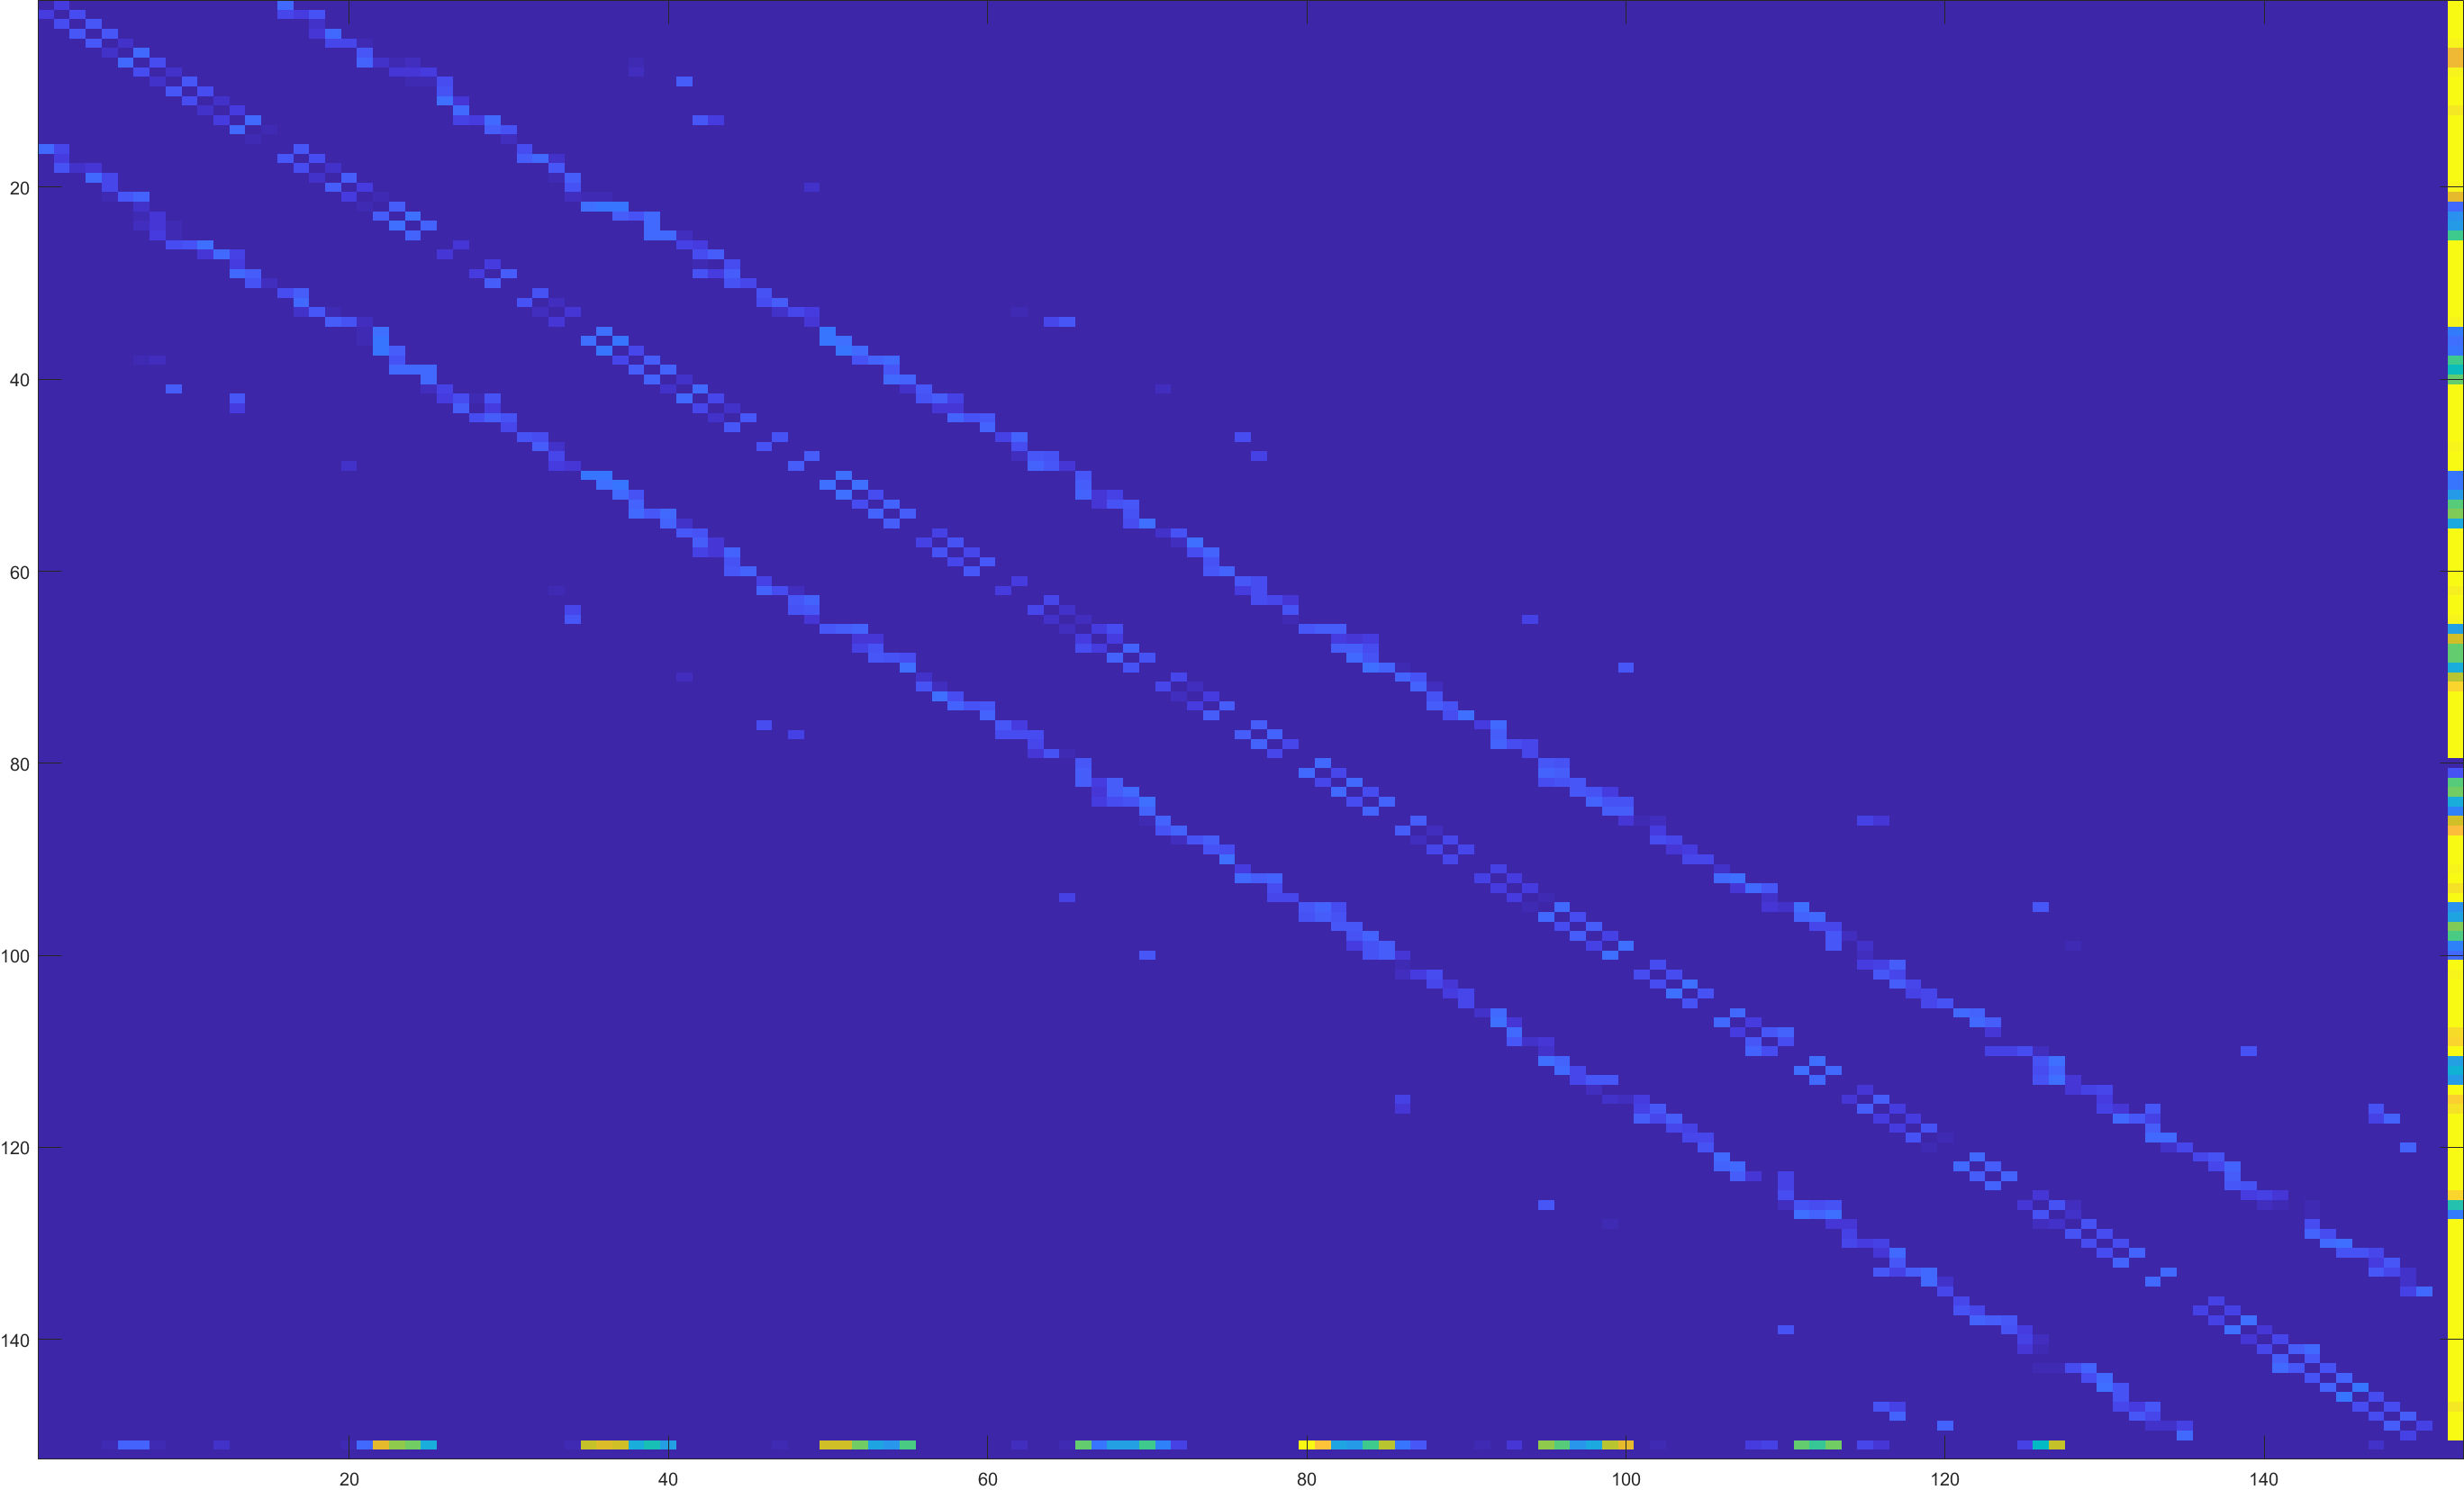
\includegraphics[width=0.8\textwidth]{hw5/capacity.png}
    \caption{Graph cut \href{./hw5/capacity.png}{capacity.png}}
    \label{fig:20}
\end{figure}

\subsubsection{Downweighted Capacity between Adjacent Nodes}
The capacities between adjacent nodes are downweighted because we want to restrict the flow relatively close to the selected superpixel as the source.
If not multiplied by 0.25, most of the superpixels may be reachable, resulting in too many foreground superpixels.
Also, it encourages the flow to reach the non-adjacent superpixels.
For this specific image, the selected superpixels are exactly the same, but they can be different for other images.


\subsection{Graph-cuts Study}
Use the \href{./hw5/example.m}{\texttt{example.m}} code here and change accordingly.
You can change other parts of the code too, if needed, but be clear to note
it.
\begin{enumerate}
    \item Run code as provided to run through a full example and show the resulting segmentation on the flower.
    Include the result.
    \item Run the code using the \href{./hw5/flag1.jpg}{flag1.jpg} image.
    Manually select a stripe on the flag.
    Are you able to get a full segmentation of the stripe and no other regions?
    If so, explain what you did to make this possible.
    If not, explain why this is hard.
    Include an rendering of the figure to substantiate your explanation either way.
    \item Run the code using the \href{./hw5/porch1.png}{porch1.png} image.
    Are you able to segment the boots perfectly?
    If so, explain what you did to make this possible.
    If not, explain why this is hard.
    Include an rendering of the figure to substantiate your explanation either way.
    \item On the \href{./hw5/porch1.png}{porch1.png} image again, are you able to segment either of the baskets perfectly?
    My guess is no.
    Can you describe (but do not implement) a way to change this system to make this more possible?
\end{enumerate}

\subsubsection{\href{./hw5/flower1.jpg}{Flower}}
The success of segmentation actually depends on the keyindex we select.
If the keyindex superpixel is not 68, then the segmentation of foreground and background are acceptable, although there are still some differencs.
If the keyindex is 68, then the segmentation fails to output.
The results are shown in Figure \ref{fig:21}, where \ref{fig:21a} is an example of successful segmentation, and \ref{fig:21b} is the example of failure.
\begin{figure}[htbp]
	\centering
	\begin{subfigure}[t]{0.8\textwidth}
	    \centering
        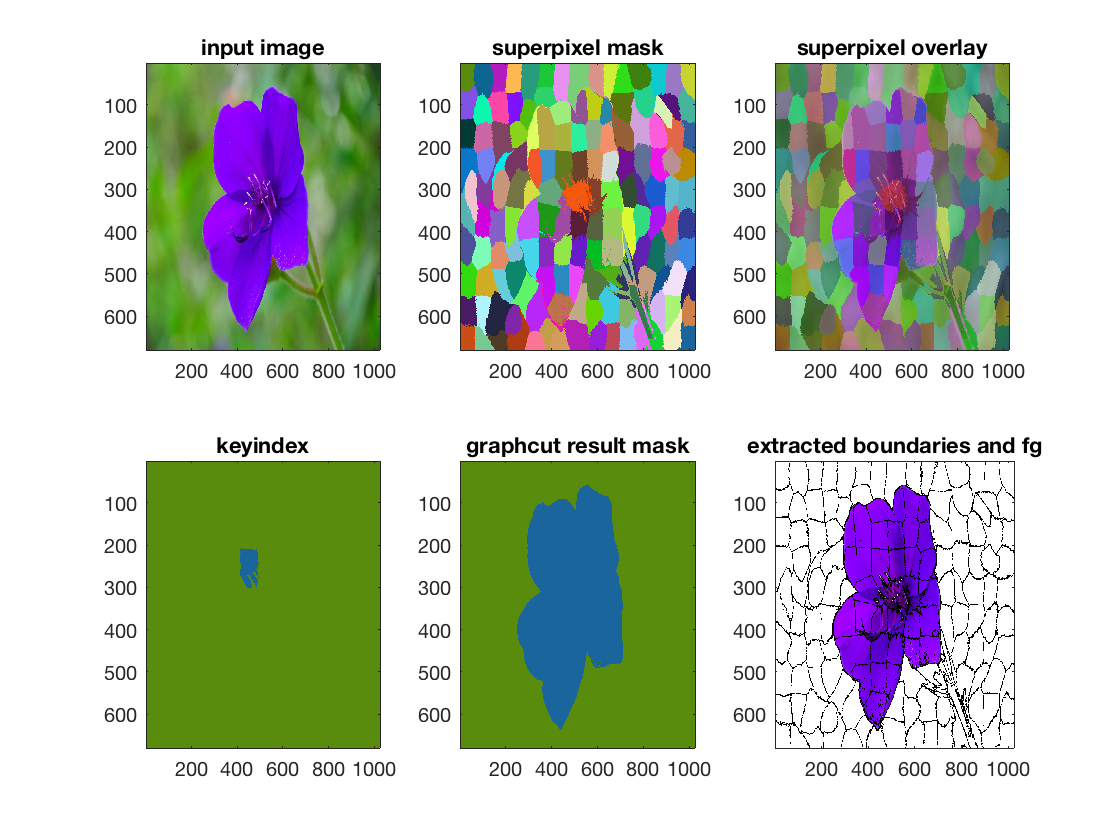
\includegraphics[width=\textwidth]{hw5/segCorrect.png}
		\caption{Successful Segmentation}\label{fig:21a}
	\end{subfigure}
	\begin{subfigure}[t]{0.8\textwidth}
	    \centering
		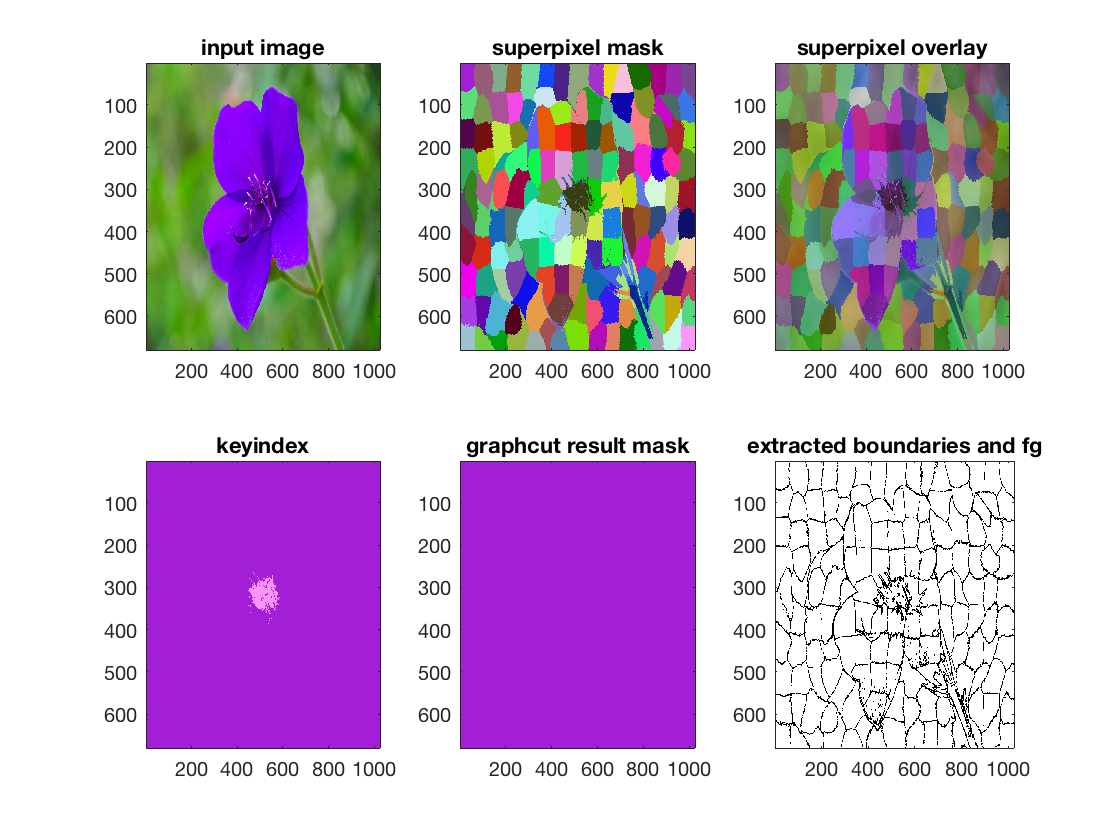
\includegraphics[width=\textwidth]{hw5/segFail.png}
		\caption{Failed Segmentation}\label{fig:21b}
	\end{subfigure}
	\caption{Segmentation on Flower Correctness Depends on Keyindex}\label{fig:21}
\end{figure}


\subsubsection{\href{./hw5/flag1.jpg}{Flag}}
The segmentation on the flag fails for almost all the keyindeces.
I tried 6 of them, and the results are in Figure \ref{fig:22}.
None of them can get all the stripes and no other regions.
Some of them manage to get the partial stripes of the selected color, while some of them even include the stars and the sky.
This is because the flag has wrinkles and shadows break the segmentation and the graph-cut algorithm choose to flow through some of the superpixels that are not stripes.
Also, since the flow cannot exceed the upper bound, most of the superpixels that are indeed strips are not flowed because the flow has already reach the capacity before flowing to them.
\begin{figure}[htbp]
	\centering
    \begin{subfigure}[t]{0.49\textwidth}
        \centering
        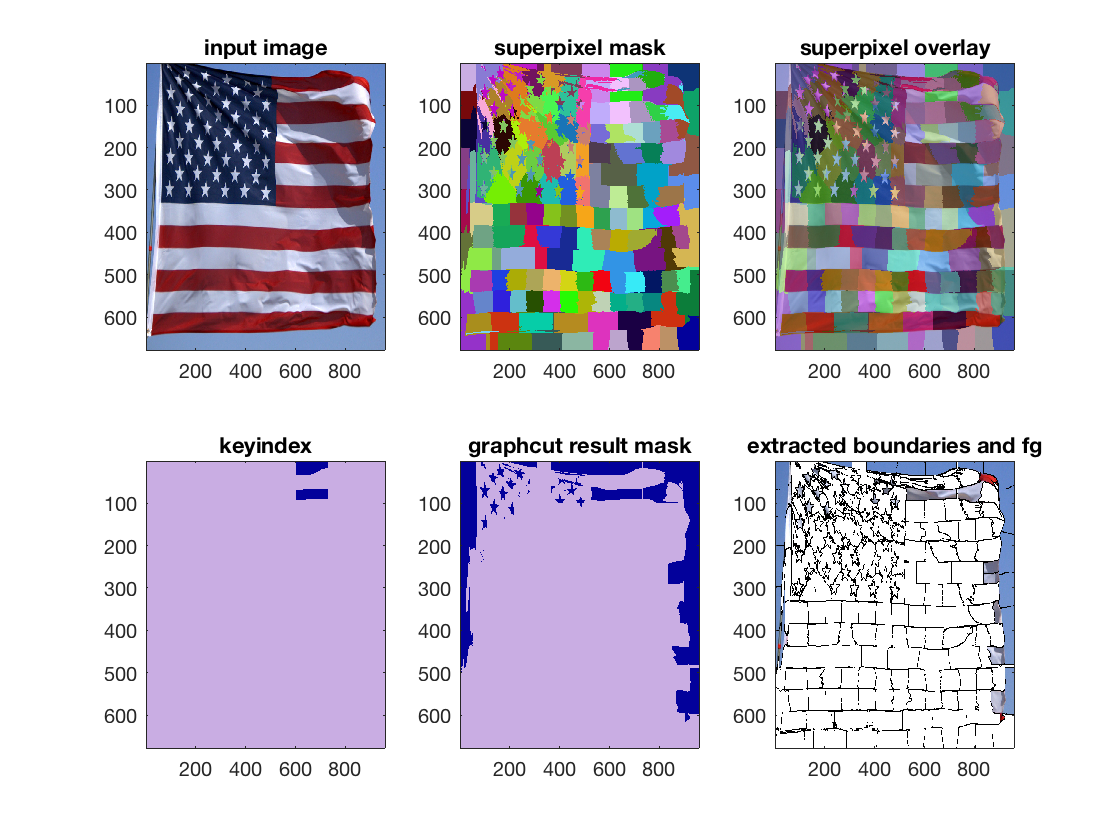
\includegraphics[width=\textwidth]{hw5/flag5.png}
		\caption{keyindex 10}\label{fig:22a}
    \end{subfigure}
    \begin{subfigure}[t]{0.49\textwidth}
        \centering
        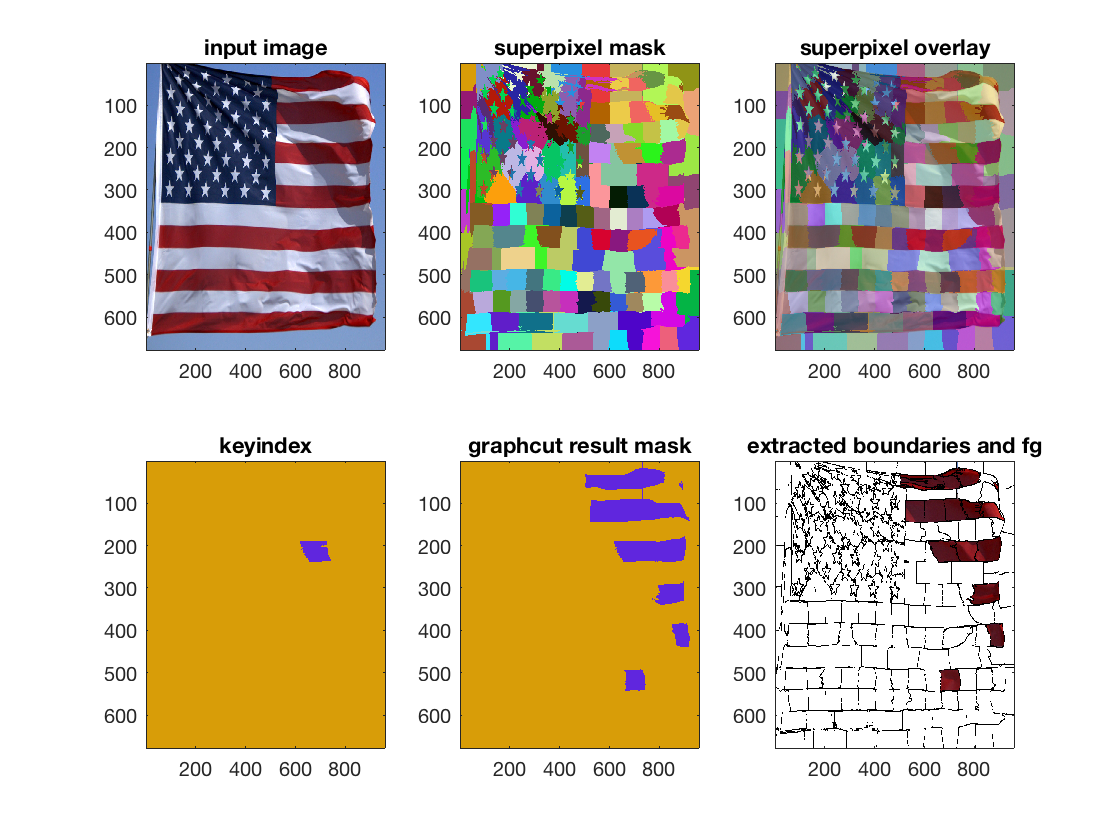
\includegraphics[width=\textwidth]{hw5/flag4.png}
		\caption{keyindex 53}\label{fig:22b}
    \end{subfigure}
    \begin{subfigure}[t]{0.49\textwidth}
        \centering
        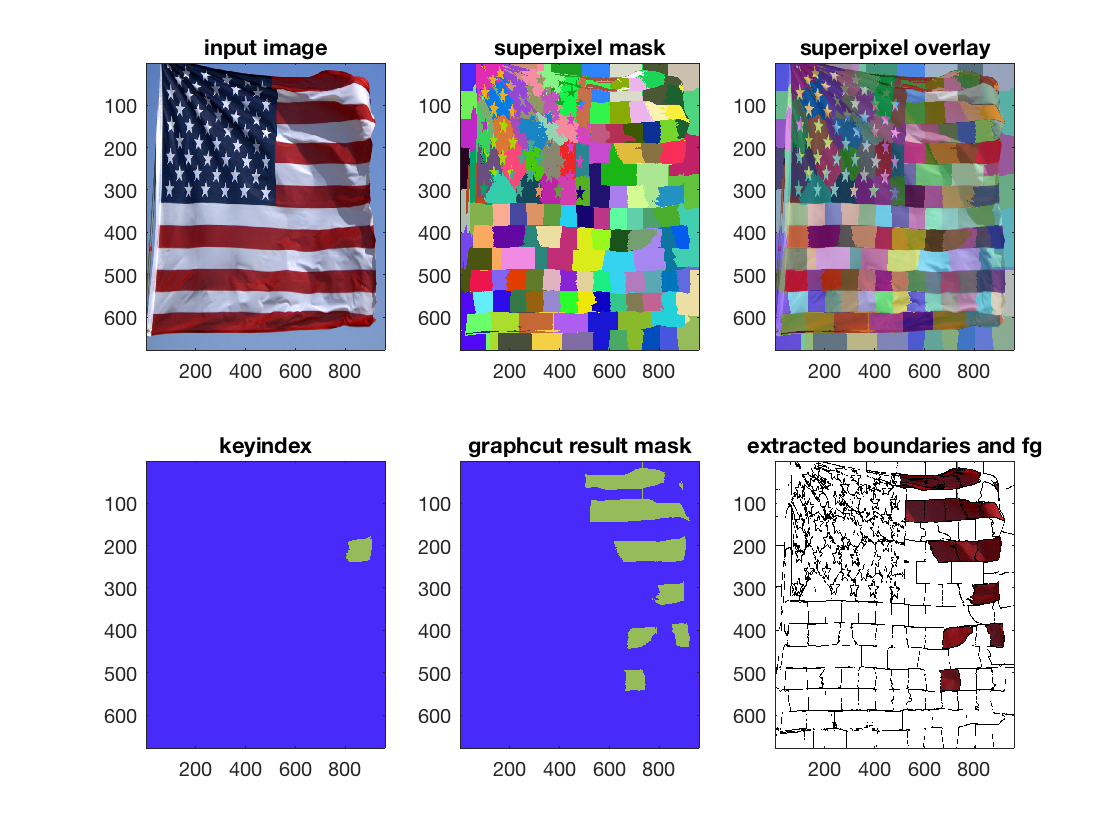
\includegraphics[width=\textwidth]{hw5/flag6.png}
		\caption{keyindex 55}\label{fig:22c}
    \end{subfigure}
    \begin{subfigure}[t]{0.49\textwidth}
        \centering
        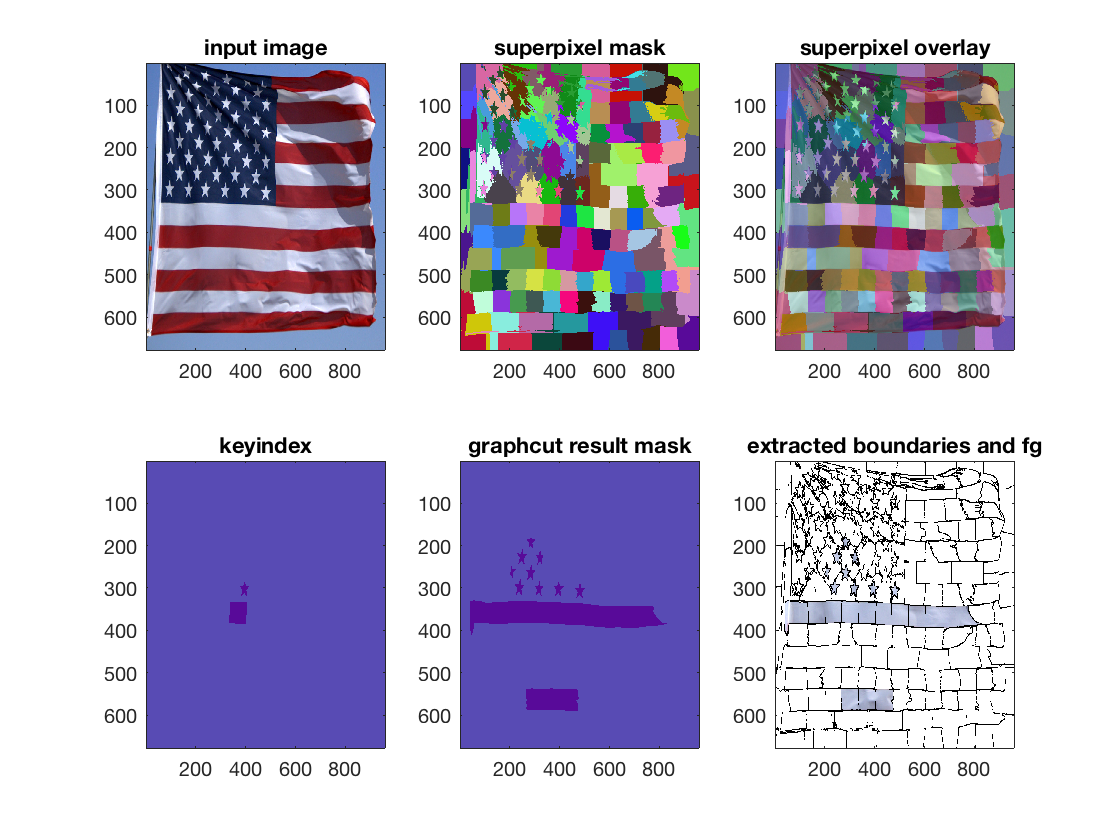
\includegraphics[width=\textwidth]{hw5/flag3.png}
		\caption{keyindex 76}\label{fig:22d}
    \end{subfigure}
    \begin{subfigure}[t]{0.49\textwidth}
	    \centering
        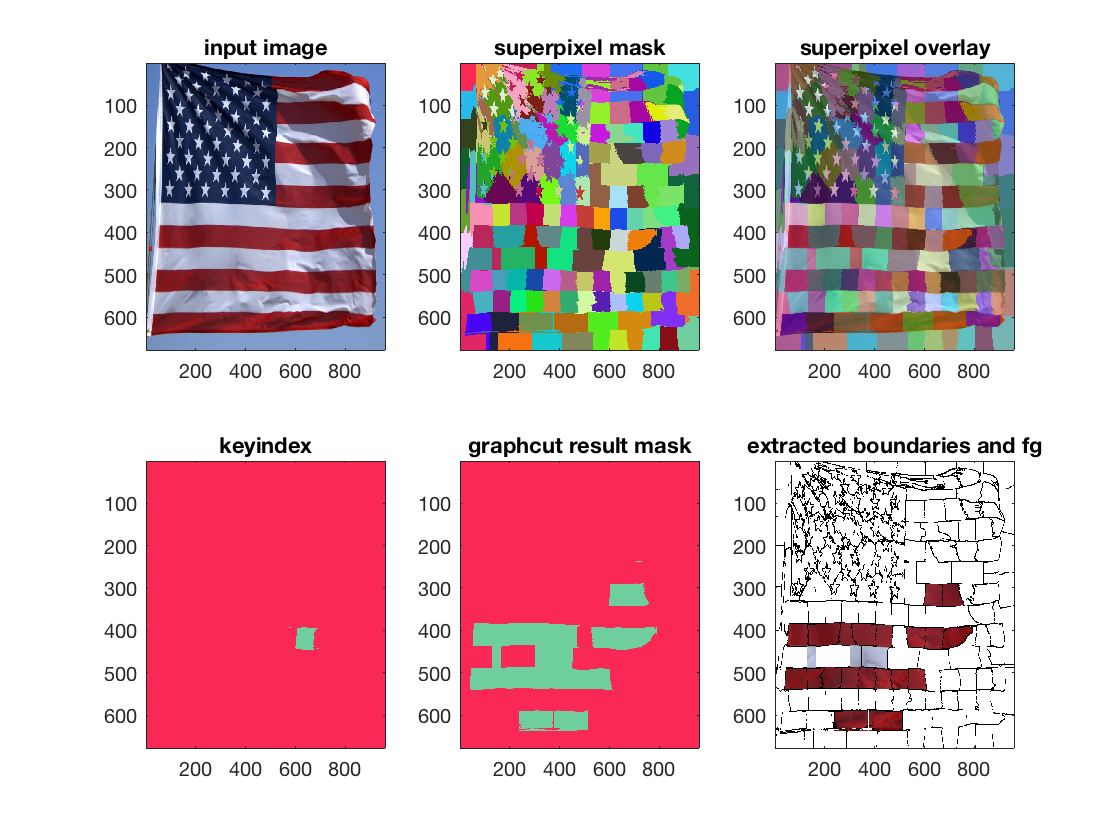
\includegraphics[width=\textwidth]{hw5/flag1.png}
		\caption{keyindex 94}\label{fig:22e}
    \end{subfigure}
    \begin{subfigure}[t]{0.49\textwidth}
	    \centering
        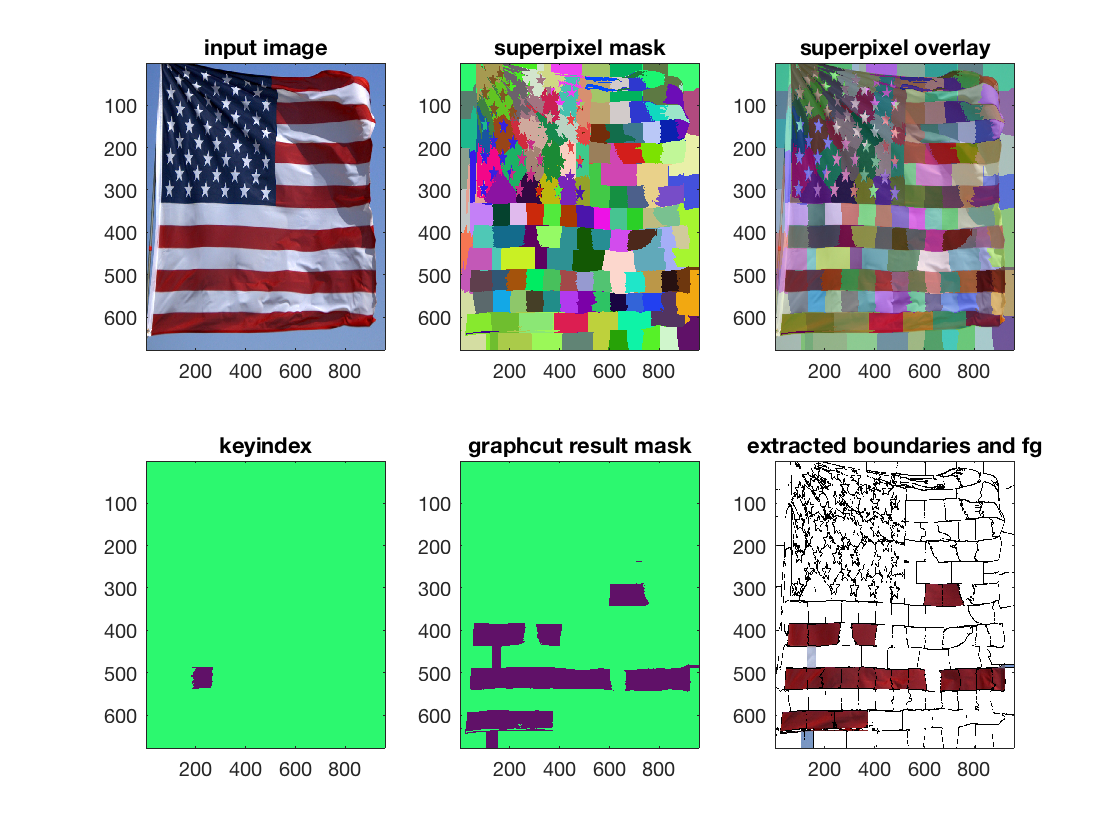
\includegraphics[width=\textwidth]{hw5/flag2.png}
		\caption{keyindex 102}\label{fig:22f}
    \end{subfigure}
    \caption{Failure of Segmentation on Flag on all Keyindex}
    \label{fig:22}
\end{figure}


\subsubsection{\href{./hw5/porch1.png}{Porch}}
Again, the success of the segmentation of the boots also depends on the keyindex, as shown in Figure \ref{fig:23}.
If the keyindex is the superpixel that represents the yellow part of the boots, then the segmentation is almost correct.
While if the keyindex is the superpixel that represents the stars on the boots, then the segmentation result is poor.
\begin{figure}[htbp]
	\centering
    \begin{subfigure}[t]{0.84\textwidth}
        \centering
        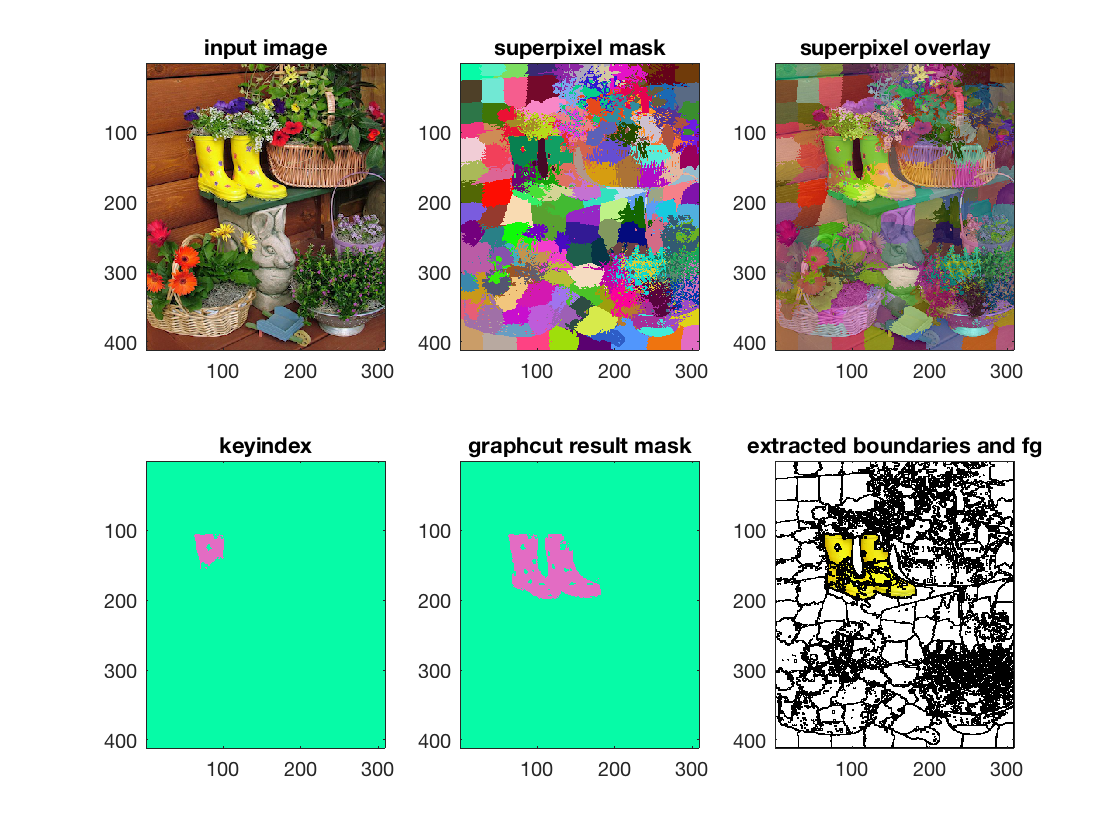
\includegraphics[width=\textwidth]{hw5/boots2.png}
		\caption{keyindex 47}\label{fig:23a}
    \end{subfigure}
    \begin{subfigure}[t]{0.84\textwidth}
        \centering
        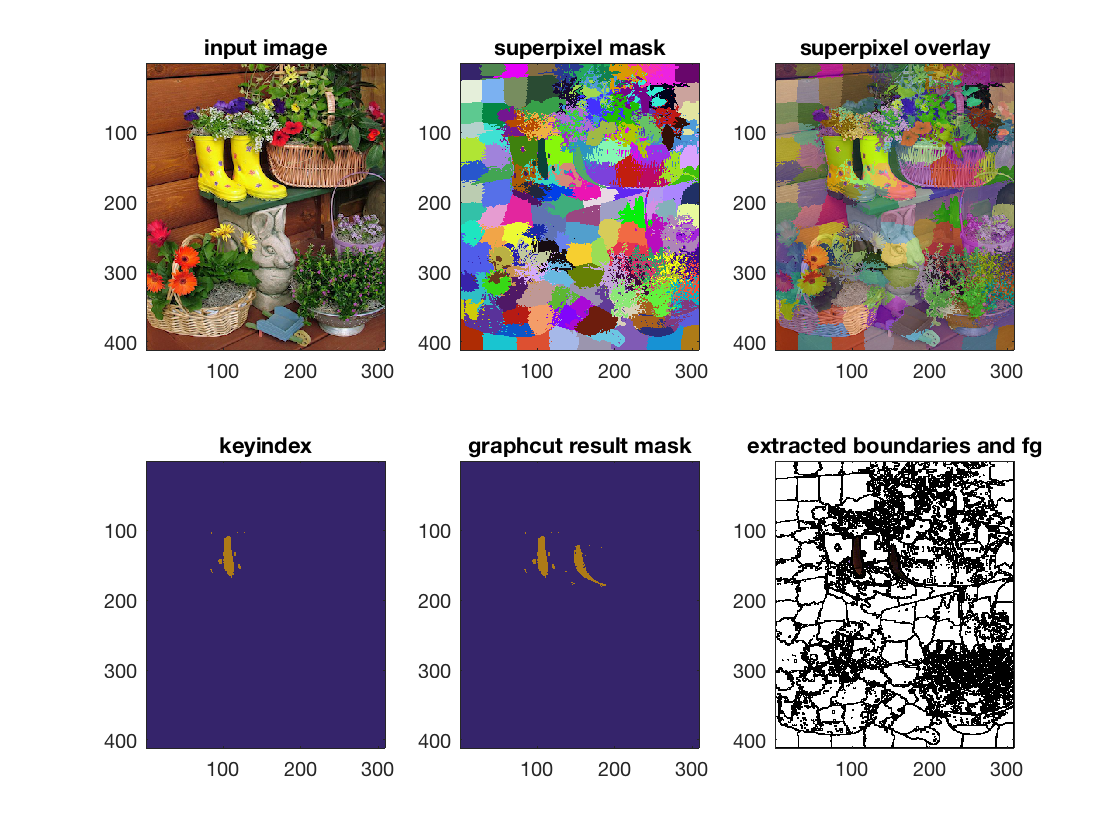
\includegraphics[width=\textwidth]{hw5/boots1.png}
		\caption{keyindex 48}\label{fig:23b}
    \end{subfigure}
    \caption{Segmentation on Boots Depends Correctness on Keyindex}
    \label{fig:23}
\end{figure}


\subsubsection{Failure of segmentation}
Again, the success of the segmentation of the baskets also depends on the keyindex, as shown in Figure \ref{fig:24}.
If the keyindex is near the upper left basket, then the segmentation is almost correct, and both of the baskets are recognized.
While if the keyindex is near the bottom left, then the segmentation includes the statue in the middle, which is not correct.
One of the reason is that the comparison depends on the difference in histogram, so segments of similar color are more likely to be together, and the low weight on adjacency also provides advantages to non-adjacent superpixels that have similar colors.
One way to improve the result is to increase the weight of the adjacent superpixels, so the superpixels that are adjacent or closer to the source are weighted more, and the non-adjacent superpixels will have less advantage in capacity, then the algorithm is more likely to generate connected superpixels.
\begin{figure}[htbp]
	\centering
    \begin{subfigure}[t]{0.84\textwidth}
        \centering
        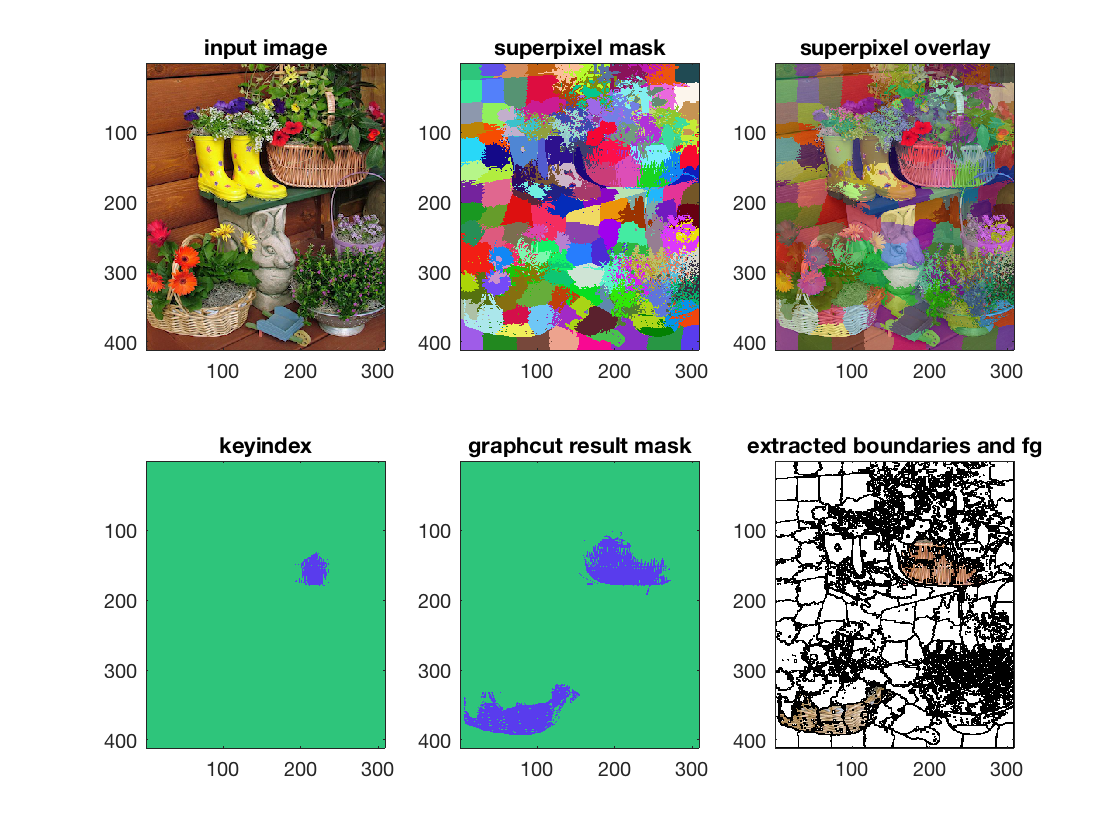
\includegraphics[width=\textwidth]{hw5/basket1.png}
		\caption{keyindex 63}\label{fig:24a}
    \end{subfigure}
    \begin{subfigure}[t]{0.84\textwidth}
        \centering
        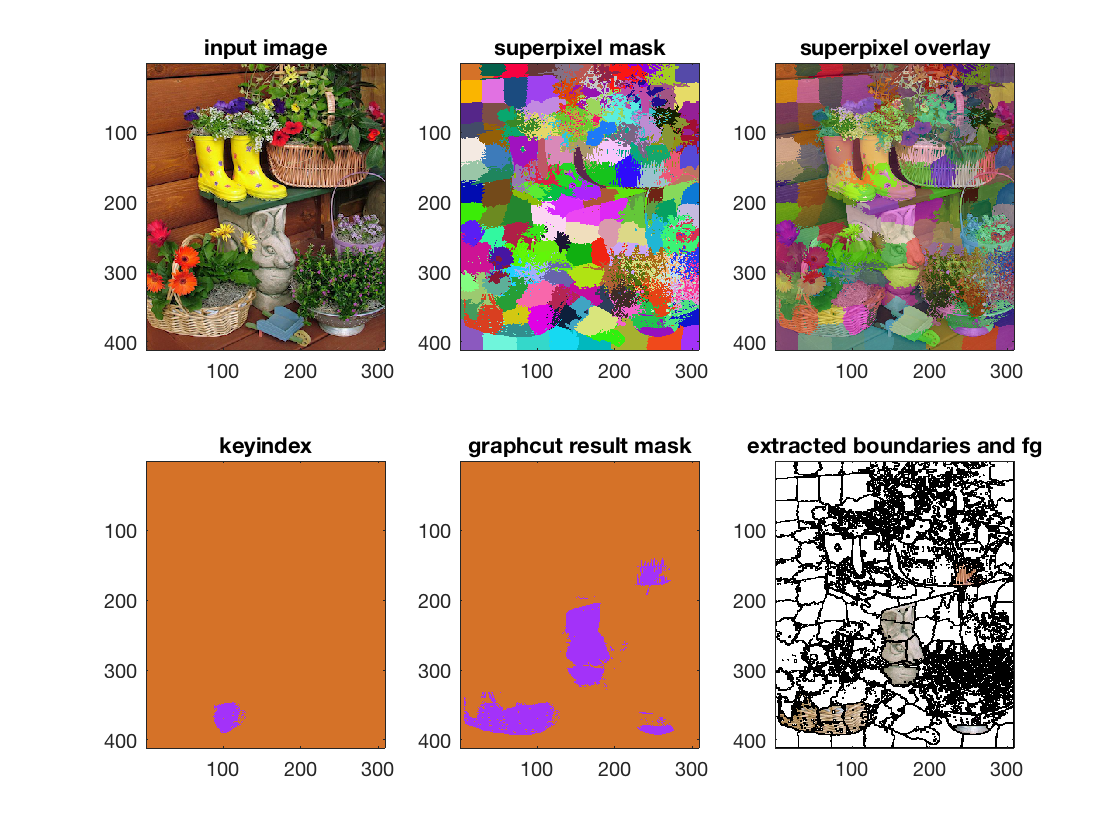
\includegraphics[width=\textwidth]{hw5/basket2.png}
		\caption{keyindex 136}\label{fig:24b}
    \end{subfigure}
    \caption{Segmentation on Baskets Correctness  Depends on Keyindex}
    \label{fig:24}
\end{figure}